\documentclass[t]{beamer}
\usetheme[deutsch]{KIT}
\setbeamercovered{transparent}
\setbeamertemplate{navigation symbols}{}

\KITfoot{Tutoriumsmaterial von Michael Vollmer}
\usepackage[utf8]{inputenc}
\usepackage{amsmath}
\usepackage{ifthen}
\usepackage{amssymb}
\usepackage{tikz}
\usepackage{ngerman}
\usepackage[normalem]{ulem}
\usepackage{stmaryrd}
\usetikzlibrary{automata}
\usenavigationsymbols
\usepackage{mathtools}
\usepackage{array}
\usepackage{colortbl}

\title{Theoretische Grundlagen der Informatik}
\subtitle{Tutorium}
\author{Michael Vollmer}

\institute[IKS]{Institut für Kryptographie und Sicherheit}

\TitleImage[height=\titleimageht]{images/tmaschine.png}

\newcommand{\N}{\ensuremath{\mathbb{N}}}
\newcommand{\M}{\ensuremath{\mathcal{M}}}
\newcommand{\classP}{\ensuremath{\mathcal{P}}}
\newcommand{\classNP}{\ensuremath{\mathcal{NP}}}
\newcommand{\co}{\ensuremath{\mathsf{co\text{-}}}}
\newcommand{\pot}{\ensuremath{\mathcal{P}}}
\newcommand{\abs}[1]{\ensuremath{\left\vert #1 \right\vert}}
\newcommand{\menge}[2]{\ensuremath{\left\lbrace #1 \,\middle\vert\, #2 \right\rbrace}}
\newcommand{\ducttape}[1]{\vspace{#1}}
\newcommand{\neglit}[1]{\overline{#1\vphantom{x^a}}}
\newcommand{\recipe}{\raisebox{-.3cm}{
\includegraphics[scale=.15]{images/chefs-cap.png}}\hspace{0.2cm}}
\newcommand{\opt}[1]{\ensuremath{\text{OPT}(#1)}}
\newcommand{\A}[1]{\ensuremath{\mathcal{A}(#1)}}
\renewcommand{\O}[1]{\ensuremath{\mathcal{O}(#1)}}
\newcommand{\msout}[1]{\text{\sout{\ensuremath{#1}}}}

\newcommand{\invincible}{\setbeamercovered{invisible}} %  "Yesss! I am invincible!!" (Boris Grishenko)
\newcommand{\vincible}{\setbeamercovered{transparent}}
\renewcommand{\solution}[1]{\invincible \pause #1 \vincible}
\newcommand{\micropause}{\\[8pt]}

% \@ifundefined{tikzset}{}{\tikzset{initial text=}} % Text "start" bei Startknoten unterdrücken
\tikzstyle{every node}=[thick]
\tikzstyle{every line}=[thick]

\newcommand{\tutnr}[1]{
  \subtitle{Tutorium #1}
	\begin{frame}
		\maketitle
	\end{frame}
}

\newcommand{\uebnr}[1]{
  \subtitle{Anmerkungen zum #1. Übungsblatt}
	\begin{frame}
		\maketitle
	\end{frame}
}

\begin{document}

\newcommand{\start}[3]
{
  \draw (#1*2,#2*2) node{$#3$};
  \draw (#1*2,#2*2) circle(0.4cm);
  \draw [->] (#1*2-0.9,#2) -- (#1*2-0.4,#2);
}
\newcommand{\final}[3]
{
  \draw (#1*2,#2*2) node{$#3$};
  \draw (#1*2,#2*2) circle(0.4cm);
  \draw (#1*2,#2*2) circle(0.32cm);
}
\newcommand{\startfinal}[3]
{
  \draw (#1*2,#2*2) node{$#3$};
  \draw (#1*2,#2*2) circle(0.4cm);
  \draw (#1*2,#2*2) circle(0.32cm);
  \draw [->] (#1*2-0.9,#2) -- (#1*2-0.4,#2);
}
\newcommand{\state}[3]
{
  \draw (#1*2,#2*2) node{$#3$};
  \draw (#1*2,#2*2) circle(0.4cm);
}
\newcommand{\tol}[4]
{
  \draw (#1+#3,#2*2) node[above]{$#4$};
  \draw [->] (#1*2-0.4,#2*2) -- (#3*2+0.4,#2*2);
}
\newcommand{\tor}[4]
{
  \draw (#1+#3,#2*2) node[above]{$#4$};
  \draw [->] (#1*2+0.4,#2*2) -- (#3*2-0.4,#2*2);
}
\newcommand{\tot}[4]
{
  \draw (#1*2,#2+#3) node[right]{$#4$};
  \draw [->] (#1*2,#2*2+0.4) -- (#1*2,#3*2-0.4);
}
\newcommand{\tob}[4]
{
  \draw (#1*2,#2+#3) node[right]{$#4$};
  \draw [->] (#1*2,#2*2-0.4) -- (#1*2,#3*2+0.4);
}
\newcommand{\totl}[5]
{
  \draw (#1+#3,#2+#4) node[above right]{$#5$};
  \draw [->] (#1*2-0.283,#2*2+0.283) -- (#3*2+0.283,#4*2-0.283);
}
\newcommand{\totr}[5]
{
  \draw (#1+#3,#2+#4) node[above left]{$#5$};
  \draw [->] (#1*2+0.283,#2*2+0.283) -- (#3*2-0.283,#4*2-0.283);
}
\newcommand{\tobl}[5]
{
  \draw (#1+#3,#2+#4) node[below right]{$#5$};
  \draw [->] (#1*2-0.283,#2*2-0.283) -- (#3*2+0.283,#4*2+0.283);
}
\newcommand{\tobr}[5]
{
  \draw (#1+#3,#2+#4) node[below left]{$#5$};
  \draw [->] (#1*2+0.283,#2*2-0.283) -- (#3*2-0.283,#4*2+0.283);
}
\newcommand{\rloopl}[3]
{
  \draw (#1*2-1,#2*2) node[left]{$#3$};
  \draw [->] (#1*2-0.35,#2*2-0.2) arc (-30:-320:0.32cm);
}
\newcommand{\rloopr}[3]
{
  \draw (#1*2+1,#2*2) node[right]{$#3$};
  \draw [->] (#1*2+0.35,#2*2+0.2) arc (150:-140:0.32cm);
}
\newcommand{\rloopt}[3]
{
  \draw (#1*2,#2*2+1) node[above]{$#3$};
  \draw [->] (#1*2-0.2,#2*2+0.35) arc (240:-50:0.32cm);
}
\newcommand{\rloopb}[3]
{
  \draw (#1*2,#2*2-1) node[below]{$#3$};
  \draw [->] (#1*2+0.2,#2*2-0.35) arc (60:-230:0.32cm);
}
\newcommand{\lloopl}[3]
{
  \draw (#1*2-1,#2*2) node[left]{$#3$};
  \draw [->] (#1*2-0.35,#2*2+0.2) arc (30:320:0.32cm);
}
\newcommand{\lloopr}[3]
{
  \draw (#1*2+1,#2*2) node[right]{$#3$};
  \draw [->] (#1*2+0.35,#2*2-0.2) arc (-150:140:0.32cm);
}
\newcommand{\lloopt}[3]
{
  \draw (#1*2,#2*2+1) node[above]{$#3$};
  \draw [->] (#1*2+0.2,#2*2+0.35) arc (-60:230:0.32cm);
}
\newcommand{\lloopb}[3]
{
  \draw (#1*2,#2*2-1) node[below]{$#3$};
  \draw [->] (#1*2-0.2,#2*2-0.35) arc (-240:50:0.32cm);
}
\tutnr{4}

\section{CYK}
\subsection{CYK-Algorithmus}

\begin{frame}
\frametitle{CYK Abschluss}
\begin{center}
\begin{tabular}{lll}
$S'\rightarrow S\mid \epsilon$&${\only<8-9,16>{\color{red}}D} \rightarrow {\only<16>{\color{red}}DD}\mid {\only<8-9>{\color{red}}d}$&${\only<6-7>{\color{red}}C} \rightarrow {\only<6-7>{\color{red}}c}$\\
${\only<13,37,69,80,85,92>{\color{red}}S} \rightarrow {\only<69,80,85,92>{\color{red}}XD}\mid {\only<13,37>{\color{red}}YC}$&${\only<13,37>{\color{red}}M}\rightarrow {\only<13,37>{\color{red}}YC}$&${\only<2-3,10,48,61>{\color{red}}X} \rightarrow {\only<48,61>{\color{red}}AM} \mid {\only<10>{\color{red}}AA} \mid {\only<2-3>{\color{red}}a}$\\
${\only<2-3,10>{\color{red}}A} \rightarrow {\only<10>{\color{red}}AA}\mid {\only<2-3>{\color{red}}a}$&${\only<4-5>{\color{red}}B} \rightarrow {\only<4-5>{\color{red}}b}$&${\only<4-5,21>{\color{red}}Y} \rightarrow {\only<21>{\color{red}}BM} \mid {\only<4-5>{\color{red}}b}$\\
\end{tabular}
\end{center}

\begin{center}
\begin{tabular}{|*{9}{C{20 pt}|}}
\hline
&{\only<2>{\color{red}}a}&{\only<3>{\color{red}}a}&{\only<4>{\color{red}}b}&{\only<5>{\color{red}}b}&{\only<6>{\color{red}}c}&{\only<7>{\color{red}}c}&{\only<8>{\color{red}}d}&{\only<9>{\color{red}}d}\\
\hline
{\only<2>{\color{red}}a}&\only<2>{\greenCell}\only<10,17,29,44,60,75,87>{\RedCell}\only<18,30-31>{\redCell}\only<2->{A,X}&\only<10>{\greenCell}\only<18,30,45,61,76,88>{\RedCell}\only<31>{\redCell}\only<10->{A,X}&\only<17-18>{\greenCell}\only<31,46,62,77,89>{\RedCell}&\only<29-31>{\greenCell}\only<47,63,78,90>{\RedCell}&\only<44-47>{\greenCell}\only<64,79,91>{\RedCell}&\only<60-64>{\greenCell}\only<80,92>{\RedCell}\only<61->{X}&\only<75-80>{\greenCell}\only<93>{\RedCell}\only<80->{S}&\only<87-94>{\greenCell}\only<92->{S}\\
\hline
{\only<3>{\color{red}}a}&\blackCell&\only<3>{\greenCell}\only<10-11,19,32,48,65,81>{\RedCell}\only<17-18,20,29-31,33-34>{\redCell}\only<3->{A,X}&\only<11>{\greenCell}\only<29,31,34>{\redCell}\only<17,20,33,49,66,82>{\RedCell}&\only<19-20>{\greenCell}\only<29,34,50,67,83>{\RedCell}&\only<32-34>{\greenCell}\only<44,51,68,84>{\RedCell}&\only<48-51>{\greenCell}\only<60,69,85>{\RedCell}\only<48->{X}&\only<65-69>{\greenCell}\only<75,86>{\RedCell}\only<69->{S}&\only<81-86>{\greenCell}\only<87>{\RedCell}\only<85->{S}\\
\hline
{\only<4>{\color{red}}b}&\blackCell&\blackCell&\only<4>{\greenCell}\only<11-12>{\RedCell}\only<17,19-20,22,29-34,36-37>{\redCell}\only<18,21,35,52,70>{\RedCell}\only<4->{B,Y}&\only<12>{\greenCell}\only<19,22,30,36,53,71>{\RedCell}\only<29,32,34,37>{\redCell}&\only<21-22>{\greenCell}\only<32,37,45,54,72>{\RedCell}\only<21->{Y}&\only<35-37>{\greenCell}\only<48,55,61,73>{\RedCell}\only<37->{S,M}&\only<52-55>{\greenCell}\only<65,74,76>{\RedCell}&\only<70-74>{\greenCell}\only<81,88>{\RedCell}\\
\hline
{\only<5>{\color{red}}b}&\blackCell&\blackCell&\blackCell&\only<5>{\greenCell}\only<12-13,20,23,31,38,56>{\RedCell}\only<19,21-22,24,29-30,32-37,39-40>{\redCell}\only<5->{B,Y}&\only<13>{\greenCell}\only<21,24,33,39,46,57>{\RedCell}\only<32,35,37,40>{\redCell}\only<13->{S,M}&\only<23-24>{\greenCell}\only<35,40,49,58,62>{\RedCell}&\only<38-40>{\greenCell}\only<52,59,66,77>{\RedCell}&\only<56-59>{\greenCell}\only<70,82,89>{\RedCell}\\
\hline
{\only<6>{\color{red}}c}&\blackCell&\blackCell&\blackCell&\blackCell&\only<6>{\greenCell}\only<13-14,22,25,34,41,47>{\RedCell}\only<21,23-24,26,32-33,35-40,42-43>{\redCell}\only<6->{C}&\only<14>{\greenCell}\only<23,26,36,42,50,63>{\RedCell}\only<35,38,40,43>{\redCell}&\only<25-26>{\greenCell}\only<38,43,53,67,78>{\RedCell}&\only<41-43>{\greenCell}\only<56,71,83,90>{\RedCell}\\
\hline
{\only<7>{\color{red}}c}&\blackCell&\blackCell&\blackCell&\blackCell&\blackCell&\only<7>{\greenCell}\only<14-15,24,27,37,51,64>{\RedCell}\only<23,25-26,28,35-36,38-43>{\redCell}\only<7->{C}&\only<15>{\greenCell}\only<25,28,39,54,68,79>{\RedCell}\only<38,41,43>{\redCell}&\only<27-28>{\greenCell}\only<41,57,72,84,91>{\RedCell}\\
\hline
{\only<8>{\color{red}}d}&\blackCell&\blackCell&\blackCell&\blackCell&\blackCell&\blackCell&\only<8>{\greenCell}\only<15-16,26,40,55,69,80>{\RedCell}\only<25,27-28,38-39,41-43>{\redCell}\only<8->{D}&\only<16>{\greenCell}\only<41>{\redCell}\only<27,42,58,73,85,92>{\RedCell}\only<16->{D}\\
\hline
{\only<9>{\color{red}}d}&\blackCell&\blackCell&\blackCell&\blackCell&\blackCell&\blackCell&\blackCell&\only<9>{\greenCell}\only<16,28,43,59,74,86,93>{\RedCell}\only<27,41-42>{\redCell}\only<9->{D}\\
\hline
\multicolumn{1}{c}{}\\
\end{tabular}

\only<94>{Sind die Wörter $abbcc$ und $abcdd$ in der Sprache der Grammatik?}
\end{center}
\end{frame}

\section{Kellerautomaten}
\subsection{Kellerautomaten}
\begin{frame}
	\frametitle{Definition Kellerautomaten}
	Ein (nichtdeterministischer) \textbf{Kellerautomat} (NPDA bzw PDA, Pushdown Automaton) besteht aus $(Q, \Sigma, \Gamma, q_0,\delta, F)$, wobei
	\begin{itemize}
		\item $Q$ endliche Zustandsmenge
		\item $\Sigma$ endliches Eingabealphabet
		\item $\Gamma$ endliches Stack-Alphabet
		\item $q_0 \in Q$ Anfangszustand
		\item $\delta : Q \times ( \Sigma \cup \{\epsilon\}) \times \Gamma \rightarrow 2^{Q \times \Gamma^*}$
		\begin{itemize}
			\item $\delta(q, a, Z) \subseteq \{(q,\gamma) : q \in Q, \gamma \in \Gamma^*\}$
			\item $\delta(q, \epsilon, Z) \subseteq \{(q,\gamma) : q \in Q, \gamma \in \Gamma^*\}$
		\end{itemize}
		\item $F \subseteq Q$ Menge der akzeptierenden Endzustände, $F=\emptyset$ ist möglich.
		
		\vspace{-4cm}\raggedleft{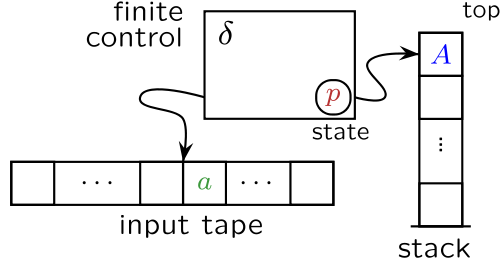
\includegraphics[width=0.5\textwidth]{images/PDA.png}}
	\end{itemize}
\end{frame}

\begin{frame}
\frametitle{Zu Kellerautomaten}
\begin{itemize}
\item Akzeptieren nach Eingabeende, wenn \begin{itemize}
	\item der Stack leer ist \emph{oder}
	\item der Automat in einen akzeptierenden Zustand kommt.
\end{itemize}
\item Sind im Allgemeinen nichtdeterministisch
\item Man kann Endzustände auch aus der Definition weglassen und alternativ verlangen, dass der Automat genau bei leerem Keller akzeptiert.
\item Man kann sogar alle Zustände bis auf einen weglassen und alles in die Kellerbelegung kodieren
\end{itemize}
\end{frame}

\begin{frame}
	\frametitle{Beispiel}
	$M = (Q, \Sigma, \Gamma, q_0, \delta, F)$
	\begin{itemize}
		\item $Q = \{q_0, q_1, q_2\}$
		\item $\Sigma = \{a,b\}$
		\item $\Gamma = \{\#,X\}$
		\item $F = \{q_2\}$
	\end{itemize}
	\begin{figure}
		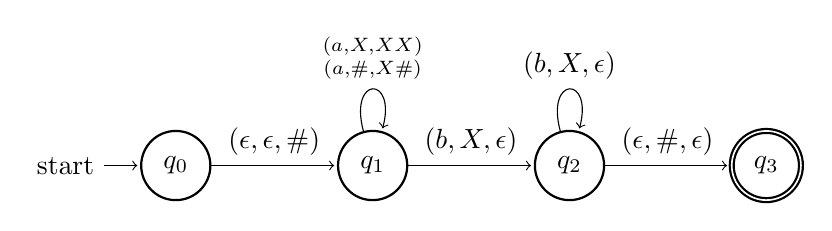
\begin{tikzpicture}[node distance=2.5cm,shorten >=1pt,auto]
			\node[state,initial]   (q_0)                {$q_0$};
			\node[state]           (q_1) [right of=q_0] {$q_1$};
			\node[state]           (q_2) [right of=q_1] {$q_2$};
			\node[state,accepting] (q_3) [right of=q_2] {$q_3$};
			\path[->]	
			(q_0) 	edge 			node {$(\epsilon,\epsilon,\#)$}				(q_1)	
			(q_1) 	edge 			node {$(b,X,\epsilon)$}				(q_2)
			edge [loop above]	node {${(a,X,XX)} \atop {(a,\#,X\#)}$}	 	()
			(q_2)	edge			node {$(\epsilon,\#,\epsilon)$}			(q_3)
			edge [loop above]	node {$(b,X,\epsilon)$}				();
		\end{tikzpicture}
	\end{figure}
	\begin{itemize}
		\item Welche Sprache akzeptiert dieser Automat?
	\end{itemize}
\end{frame}

\subsection{Alte Aufgabe 3}
\begin{frame}
	\frametitle{Alte Aufgabe 3}
	Gegeben sei folgende Sprache f"ur das Alphabet $\Sigma = \{a,b,c\}$:
	\begin{multline*}
		\mathcal{L} = \{w_1w_2 \in \Sigma^* \; | \; w_1 \in \{a,b\}^*,w_2 \in \{b,c\}^*,\\
		\#_a w_1 + \#_b w_1 = \#_b w_2 + \#_c w_2\}
	\end{multline*}
	Hier gibt $\#_x w$ die H"aufigkeit des Vorkommens eines Zeichens $x \in \Sigma$ in
	einem Wort $w \in \Sigma^*$ an.
	\begin{enumerate}
		\item Zeigen Sie, dass $\mathcal{L}$ nicht regul"ar ist!
		\item Geben Sie eine Chomsky-2-Grammatik an, die genau die Sprache $\mathcal{L}$
		erzeugt!
		\item Geben Sie einen Kellerautomaten $\mathcal{M}$ an, der genau die Sprache
		$\mathcal{L}$ erkennt! Zeichnen Sie den\\
		Zustands"ubergangsgraphen f"ur $\mathcal{M}$!
	\end{enumerate}
\end{frame}

\section{Pumping Lemma für kontextfreie Sprachen}
\subsection{Pumping Lemma für kontextfreie Sprachen}
\begin{frame}
	\frametitle{Pumping-Lemma für kontextfreie Sprachen}
	\begin{exampleblock}{Lemma}
		Für jede kontextfreie Sprache $L$ gibt es eine Konstante $n \in \mathbb{N}$,
		so dass sich jedes Wort $z \in L$ mit $|z| \geq n$ so als
		$$ z = uvwxy $$
		schreiben lässt, dass
		\begin{itemize}
			\item $|vx| \geq 1$,
			\item $|vwx| \leq n$ und
			\item für alle $i \geq 0$ das Wort $uv^iwx^iy \in L$ ist.
		\end{itemize}
	\end{exampleblock}
\end{frame}

\begin{frame}
	\frametitle{Beweisidee}
	\begin{itemize}
		\item Jeder Knoten im Ableitungsbaum (wie wir ihn in CYK sehen) steht für ein Nichtterminalsymbol
		\item Ab einer gewissen Höhe des Baumes (bzw. Länge des Wortes) muss ein Nichtterminal im Baum mehrmals in einer Reihe vorkommen
		\item Man kann also aus einem Nichtterminalsymbol dasselbe Symbol wieder ableiten
		\item Da das Wort durch jede Ableitung (außer zu Terminalsymbolen) länger wird, gibt es eine "`Schleife"' beim Ableiten
		\item Diese Schleife kann man also "`pumpen"', also beliebig oft (oder auch gar nicht) durchlaufen
	\end{itemize}
\end{frame}

\begin{frame}
	\frametitle{Beweisidee}
	\begin{figure}[H]
		\centering
		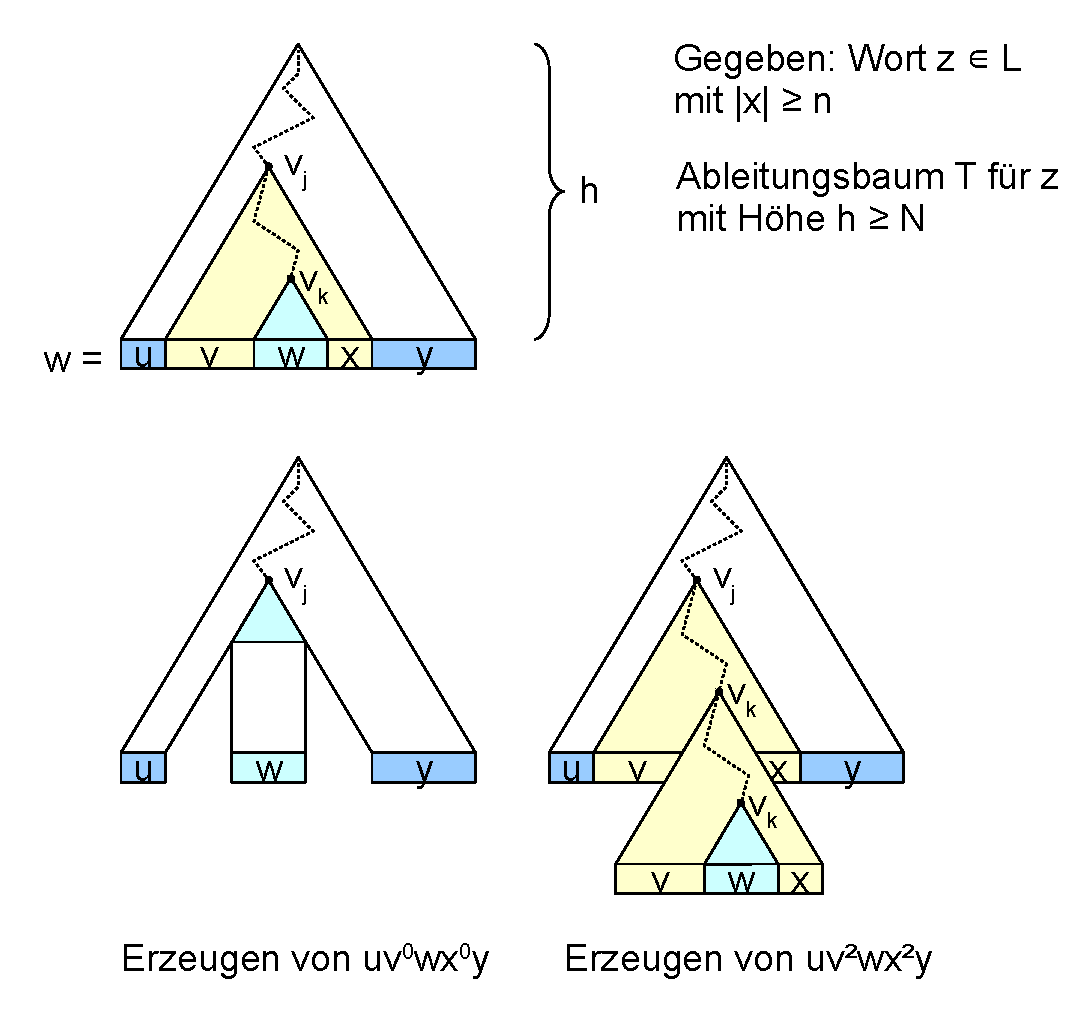
\includegraphics[scale=0.41]{images/pumping}
	\end{figure}
\end{frame}

\frame{
	\frametitle{Pumping Lemma Formalia (kontextfrei)}
	Behauptung: L ist nicht kontextfrei. ~\\
	Beweis:
	\begin{enumerate}
	\item[] Nehme an L sei kontextfrei.% Sei n wie im Pumping Lemma gefordert.
	\item[] Sei n beliebig aber fest.
	%\item Pumping Lemma: $\exists n \in N$, so dass jedes Wort $z \in L$ mit $|z| \ge n$ eine Zerlegung z = uvwxy besitzt mit $|vx|\ge 1$ und $|vwx|\le n$, so dass $uv^iwx^iy \in L$  für $\forall i\in \N_0$
	\item[] Wähle z=\underline{\hspace{3cm}} $\in L$ mit $|z| \ge n$
	%\item Zeige, dass für alle Zerlegungen von z, die den Regeln des Pumping Lemmas genügen, ein i existiert, sodass $uv^iwx^iy\not\in L$
	\item[] Beh.: $\forall u,v,w,x,y: uvwxy=z$ mit $|vx|\ge 1$ und $|vwx|\le n$, $\exists i \in N$, so dass $uv^iwx^iy \not\in L$.
	\item[] Bew.:\underline{\hspace{8cm}}
	\item[] Widerspruch zum Pumping Lemma $\Rightarrow$ L ist nicht kontextfrei.
	\end{enumerate}
}

\begin{frame}
	\frametitle{Beispiel}
	Zeige, dass die Sprache
	\[L=\{\omega \omega|\omega \in \{0,1\}^*\}\]
	nicht kontextfrei ist.
\end{frame}

\subsection{Aufgabe 1}
\begin{frame}
	\frametitle{Aufgabe 1}
	\begin{enumerate}
		\item Geben Sie f"ur die Sprache $\mathcal{L} = \{a^nb^nc^n \; | \; n \in
		\mathbb{N}\}$ eine Grammatik des h"ochstm"oglichen Chomsky-Typs an!
		\item Zeigen Sie, dass die Sprache $\mathcal{L}' = \{a^{2^n} \; | \; n \in
		\mathbb{N}\}$ nicht kontextfrei ist!
	\end{enumerate}
\end{frame}

\section{Schluss}
\subsection{Schluss}

\begin{frame}
\frametitle{Bis zum nächsten Mal!}
\begin{center}
  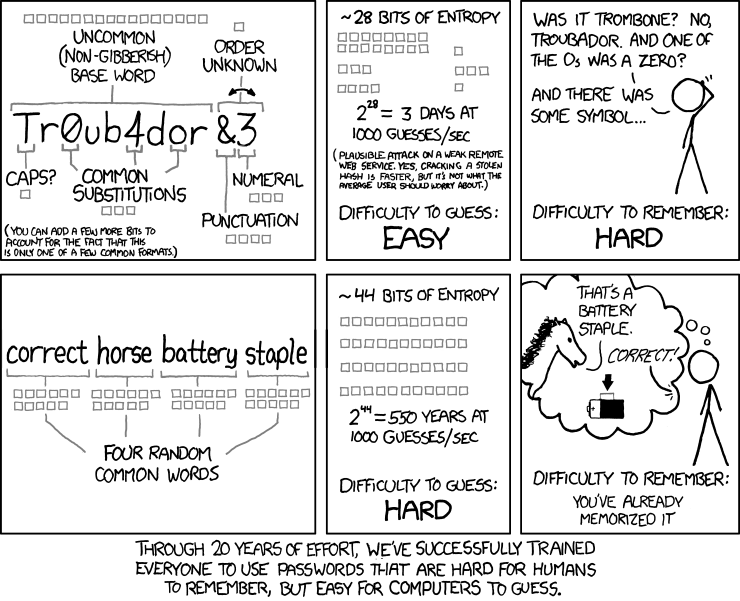
\includegraphics[width=1 \textheight]{images/password_strength.png}
\end{center}
\end{frame}

\frame{
  \frametitle{Lizenzen}
  \center
  
\includegraphics[width=2em]{images/by}
  
\includegraphics[width=2em]{images/cc}
  
\includegraphics[width=2em]{images/sa}
  \\
  {\tiny

Dieses Werk ist unter einem ``Creative Commons Namensnennung-Weitergabe unter gleichen Bedingungen 3.0 Deutschland``-Lizenzvertrag lizenziert. Um eine Kopie der Lizenz zu erhalten, gehen Sie bitte zu \href{http://creativecommons.org/licenses/by-sa/3.0/de/}{http://creativecommons.org/licenses/by-sa/3.0/de/} oder schreiben Sie an Creative Commons, 171 Second Street, Suite 300, San Francisco, California 94105, USA.\\
  \vspace{1cm}
  Davon ausgenommen sind das Titelbild, welches aus der März-April 2002 Ausgabe von American Scientist erschienen ist und ohne Erlaubnis verwendet wird, sowie das KIT Beamer Theme. Hierfür gelten die Bestimmungen der jeweiligen Urheber.
  \vspace{1cm}
  \\ 
  }
  %Habe hier die Reihenfolge etwas umgestellt, weil die Formatierung bei mir komisch aussah. 
  %Wenn es bei dir anders ist, kannst du es auch wieder zurückändern, dann haben wir unterschiedliche Kompilieroptionen
}

\end{document}